\chapter*{Dodatak: Prikaz aktivnosti grupe}
		\addcontentsline{toc}{chapter}{Dodatak: Prikaz aktivnosti grupe}
		
		\section*{Dnevnik sastajanja}
		
		\begin{packed_enum}
			\item  sastanak
			
			\item[] \begin{packed_item}
				\item Datum: 3. listopada 2019.
				\item Prisutni: I. Juren, T. Krmek, M. Jurić, M. Zec, S. Gaši, M. Nosil, P. Lanča
				\item Teme sastanka:
				\begin{packed_item}
					\item  predlaganje ideja za projektni zadatak
					\item  odabir između web ili mobilne aplikacije
					\item  svaki član je iznio koja predznanja ili iskustva ima vezano za stvaranje aplikacije  
				\end{packed_item}
			\end{packed_item}
			
			\item  sastanak
			\item[] \begin{packed_item}
				\item Datum: 9. listopada 2019.
				\item Prisutni: I. Juren, T. Krmek, M. Jurić, M. Zec, S. Gaši, M. Nosil, P. Lanča
				\item Teme sastanka:
				\begin{packed_item}
					\item  upoznavanje s mentorima i demonstratorom
					\item  razgovor o tehnologijama koje ćemo koristiti
					\item  dogovoren način komunikacije s asistentom i demonstratorom
					\item  upoznavanje s ponuđenim projektom te razgovor o tome kako poboljšati naš prijedlog projekta
				\end{packed_item}
			\end{packed_item}
			
			\item  sastanak
			\item[] \begin{packed_item}
				\item Datum: 14. listopada 2019.
				\item Prisutni: I. Juren, M. Jurić, M. Zec, S. Gaši, P. Lanča
				\item Teme sastanka:
				\begin{packed_item}
					\item  sastanak s asistentom
					\item  nacrtana gruba shema različitih korisnika s pripadajućim potrebnim pristupom
					\item  predlaganje funkcionalnosti, dogovoreno što se obavezno mora implementirati 
				\end{packed_item}
			\end{packed_item}
			
			\item  sastanak
			\item[] \begin{packed_item}
				\item Datum: 22. listopada 2019.
				\item Prisutni: I. Juren, T. Krmek, M. Jurić, M. Zec, S. Gaši, M. Nosil, P. Lanča
				\item Teme sastanka:
				\begin{packed_item}
					\item  razrada must i could have funkcionalnosti
					\item  izjašnjavanje svojih nedoumica te njihovo razrješavanje, eventualno stavljene na popis za pitanja na sastanku s asistentom
					\item  razriješena problematika benda (glavni i rezervni članovi)
					\item  nakon internog, sastanak s asistentom: dogovorena detaljnija implementacija, napravljen popis zadataka koje treba odraditi do idućeg sastanka
				\end{packed_item}
			\end{packed_item}
			
			\item  sastanak
			\item[] \begin{packed_item}
				\item Datum: 28. listopada 2019.
				\item Prisutni: I. Juren, M. Jurić, M. Zec, S. Gaši, M. Nosil, P. Lanča
				\item Teme sastanka:
				\begin{packed_item}
					\item  nabrajanje usecase-ova
					\item  podjela rada
					\item  određena pitanja za idući sastanak s asistentom
				\end{packed_item}
			\end{packed_item}
			
			\item  sastanak
			\item[] \begin{packed_item}
				\item Datum: 29. listopada 2019.
				\item Prisutni: I. Juren, M. Jurić, M. Zec, S. Gaši, M. Nosil, P. Lanča
				\item Teme sastanka:
				\begin{packed_item}
					\item  sastanak s asistentom: pokazano što je sve napravljeno
					\item  napravljen popis zadataka koji moraju biti gotovi do idućeg sastanka s asistentom i sve što još treba za prvu verziju
					\item  riješena dilema oko recenzija
					\item  razriješen problem solista, bit će jednočlani bend
					\item  rasprava oko baze podataka, što treba promijeniti i poboljšati
				\end{packed_item}
			\end{packed_item}
			
			\item  sastanak
			\item[] \begin{packed_item}
				\item Datum: 11. studenog 2019.
				\item Prisutni: I. Juren, M. Jurić, M. Zec, S. Gaši, M. Nosil, P. Lanča, T. Krmek
				\item Teme sastanka:
				\begin{packed_item}
					\item  određivanje preostalih poslova te njihov raspored po članovima
					\item  na sastanku dovršen frontend te je aplikacija isporučena
				\end{packed_item}
			\end{packed_item}
			
			\item  sastanak
			\item[] \begin{packed_item}
				\item Datum: 12. listopada 2019.
				\item Prisutni: I. Juren, M. Jurić, M. Zec, S. Gaši, M. Nosil, P. Lanča, T. Krmek
				\item Teme sastanka:
				\begin{packed_item}
					\item  sastanak s asistentom: pokazana aplikacija te dokumentacija
					\item  razriješene neke nedoumice oko baze podataka
				\end{packed_item}
			\end{packed_item}
			
			\item  sastanak
			\item[] \begin{packed_item}
				\item Datum: 10. prosinca 2019.
				\item Prisutni: I. Juren, M. Jurić, M. Zec, S. Gaši, M. Nosil, P. Lanča, T. Krmek
				\item Teme sastanka:
				\begin{packed_item}
					\item  sastanak s asistentom: razrada plana, pitanja vezana za aplikaciju
					\item  raspored poslova
				\end{packed_item}
			\end{packed_item}
			
			\item  sastanak
			\item[] \begin{packed_item}
				\item Datum: 7. siječnja 2019.
				\item Prisutni: I. Juren, M. Jurić, M. Zec, S. Gaši, M. Nosil, P. Lanča, T. Krmek
				\item Teme sastanka:
				\begin{packed_item}
					\item  sastanak s asistentom: prikaz alfa verzije, razrada daljnjeg plana, što popraviti
					\item  raspored poslova
				\end{packed_item}
			\end{packed_item}
			
			\item  sastanak
			\item[] \begin{packed_item}
				\item Datum: 7. siječnja 2019.
				\item Prisutni: I. Juren, M. Jurić, M. Zec, S. Gaši, M. Nosil, P. Lanča, T. Krmek
				\item Teme sastanka:
				\begin{packed_item}
					\item  sastanak s asistentom: pokazivanje popravaka dizajna i dodanih funkcionalnosti
					\item  raspored poslova
				\end{packed_item}
			\end{packed_item}
			
			\item  sastanak
			\item[] \begin{packed_item}
				\item Datum: 16. siječnja 2019.
				\item Prisutni: I. Juren, M. Jurić, M. Zec, S. Gaši, M. Nosil, P. Lanča, T. Krmek
				\item Teme sastanka:
				\begin{packed_item}
					\item interni sastanak i završetak radova na projektu, popravljanje i ispravljanje
				\end{packed_item}
			\end{packed_item}
			%
			
		\end{packed_enum}
		
		\eject
		\section*{Tablica aktivnosti}
			\begin{longtabu} to \textwidth {|X[7, l]|X[1, c]|X[1, c]|X[1, c]|X[1, c]|X[1, c]|X[1, c]|X[1, c]|}
								
				\cline{2-8} \multicolumn{1}{c|}{\textbf{}} &     \multicolumn{1}{c|}{\rotatebox{90}{\textbf{Ivan Juren }}} & \multicolumn{1}{c|}{\rotatebox{90}{\textbf{Stela Gaši }}} &	\multicolumn{1}{c|}{\rotatebox{90}{\textbf{Marin Jurić }}} &	\multicolumn{1}{c|}{\rotatebox{90}{\textbf{Tomislav Krmek   }}} &
				\multicolumn{1}{c|}{\rotatebox{90}{\textbf{Paolo Lanča }}} &
				\multicolumn{1}{c|}{\rotatebox{90}{\textbf{Mihael Nosil }}} &	\multicolumn{1}{c|}{\rotatebox{90}{\textbf{Mario Zec }}} \\ \hline 
				\endfirsthead
				
			
				\cline{2-8} \multicolumn{1}{c|}{\textbf{}} &     \multicolumn{1}{c|}{\rotatebox{90}{\textbf{Ivan Juren}}} & \multicolumn{1}{c|}{\rotatebox{90}{\textbf{Stela Gaši }}} &	\multicolumn{1}{c|}{\rotatebox{90}{\textbf{Marin Jurić }}} &
\multicolumn{1}{c|}{\rotatebox{90}{\textbf{Tomislav Krmek }}} &	\multicolumn{1}{c|}{\rotatebox{90}{\textbf{Paolo Lanča }}} &
\multicolumn{1}{c|}{\rotatebox{90}{\textbf{Mihael Nosil }}} &	\multicolumn{1}{c|}{\rotatebox{90}{\textbf{Mario Zec }}} \\ \hline 
				\endhead
				
				
				\endfoot
							
				 
				\endlastfoot
				
				Upravljanje projektom 		& 4 & 3 &  & 1 & 3 &  & 3 \\ \hline
				Opis projektnog zadatka 	& 3 & 2 &  &  &  &  & 1 \\ \hline
				Funkcionalni zahtjevi       & 2 & 2 &  &  &  & 1 & 2 \\ \hline
				Opis pojedinih obrazaca 	&  & 2 & 1 &  & 2 & 10 & 4 \\ \hline
				Dijagram obrazaca 			&  &  &  &  & 1 &  & 3 \\ \hline
				Sekvencijski dijagrami 		&  & 2 & 2 &  & 1 &  &  \\ \hline
				Opis ostalih zahtjeva 		&  &  & 1 &  & 1 &  &  \\ \hline
				Arhitektura i dizajn sustava	 & 6 & 2 &  &  & 2 &  &  \\ \hline
				Baza podataka				& 10 & 8 &  & 3 &  &  &   \\ \hline
				Dijagram razreda 			& 2 & 1 &  &  &  &  & 15  \\ \hline
				Dijagram stanja 			&  &  & 1 &  &  &  &   \\ \hline
				Dijagram razmještaja 			&  &  &  &  &  &   &  2 \\ \hline
				Dijagram komponenti 			&  &  &  &  &  &   &  4 \\ \hline
				Dijagram aktivnosti 		&  & 3 &  &  &  &  &  \\ \hline
				Korištene tehnologije i alati 	&  &  & 1 &  &  &   &   \\ \hline
				Ispitivanje programskog rješenja 	& 10  & 10 &  & 3  &  &   &   \\ \hline
				Upute za puštanje u pogon 			& 8 &  &  &  &  & 2  &   \\ \hline
				Zaključak i budući rad 			&  &  &  &  &  & 2  &   \\ \hline
				Dnevnik sastajanja 			& 1 & 1 &  &  & 3 &  &  \\ \hline
				Popis literature 			& 1 & 1 &  &  &  &  &  \\  \hline
				\textit{Frontend} 			& 10 &  & 55 & 70 & 60  & 50 &  \\ \hline
				\textit{Backend} 				& 100 & 40 &  &  &  &  & 40  \\ \hline
				\textit{Vrijeme provedeno na sastancima} 		 			& 15 & 15 & 15 & 7 & 10 & 9 & 10 \\ \hline 

				
				
			\end{longtabu}
					
					
		\eject
		
		\section*{Dijagrami pregleda promjena}
		
		\begin{figure}[H]
			\begin{center}
				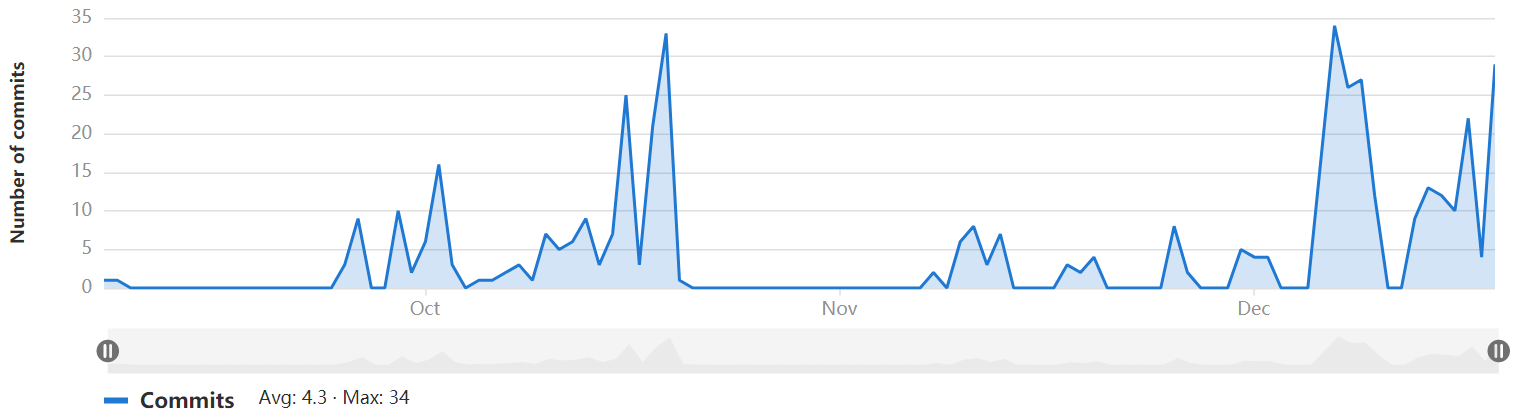
\includegraphics[width=15cm]{slike/dijagrampregledapromjena.PNG}
			\end{center}
			\caption{Dijagram pregleda promjena na grani Master}
			\label{fig:master}
		\end{figure}
		
		\begin{figure}[H]
			\begin{center}
				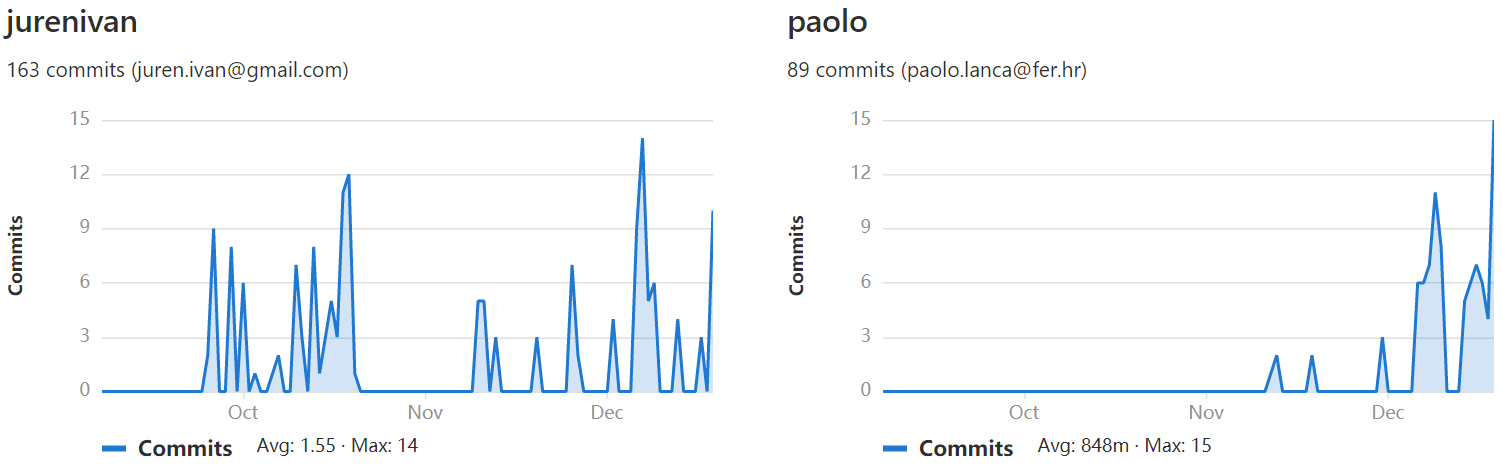
\includegraphics[width=15cm]{slike/dijagrampregledapromjena1.PNG}
				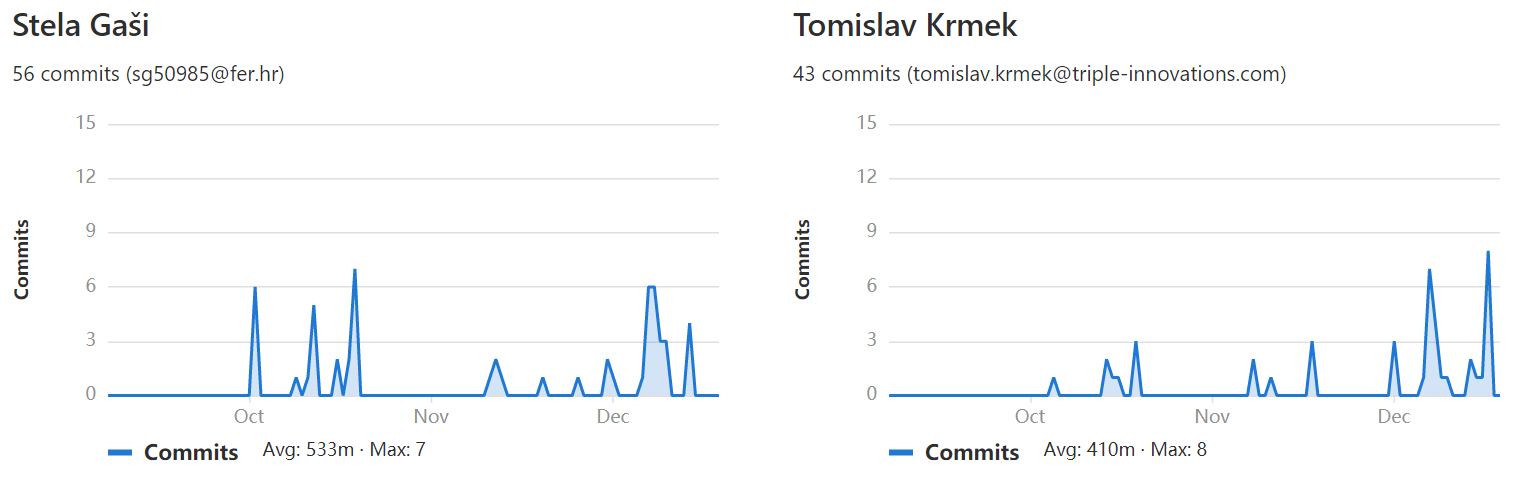
\includegraphics[width=15cm]{slike/dijagrampregledapromjena2.PNG}
				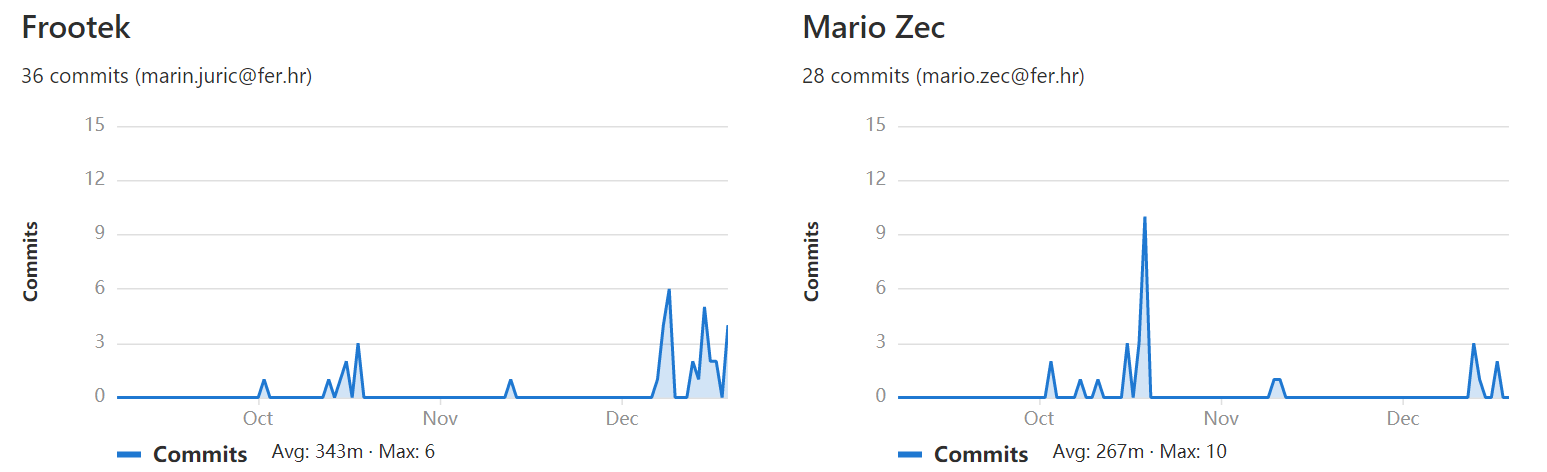
\includegraphics[width=15cm]{slike/dijagrampregledapromjena3.PNG}
				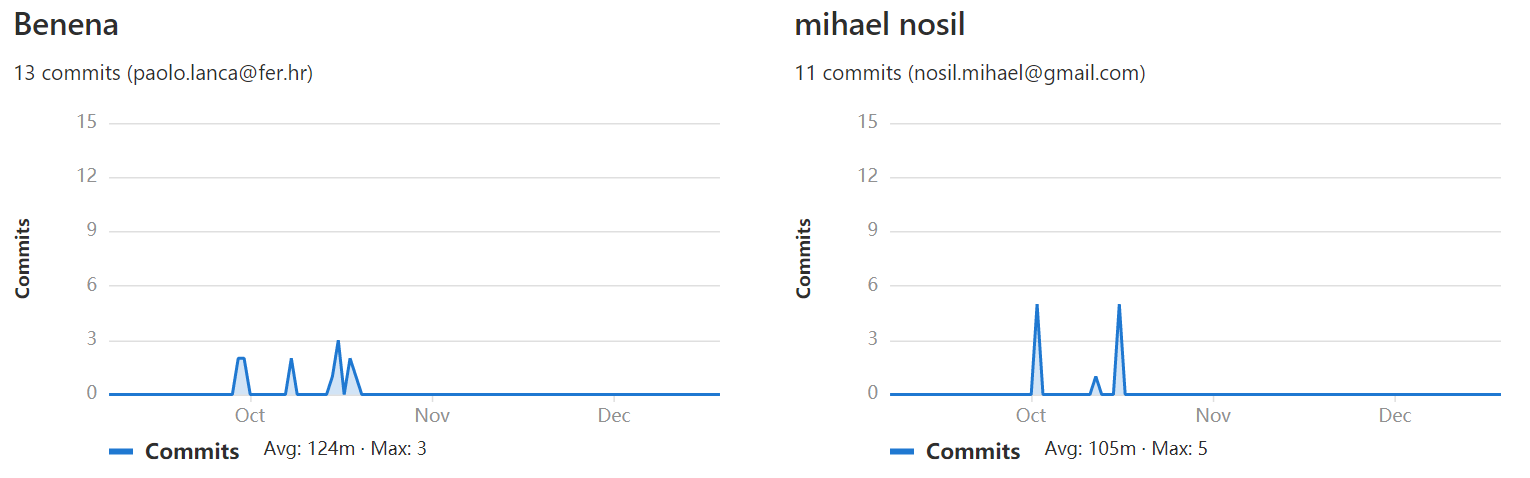
\includegraphics[width=15cm]{slike/dijagrampregledapromjena4.PNG}
				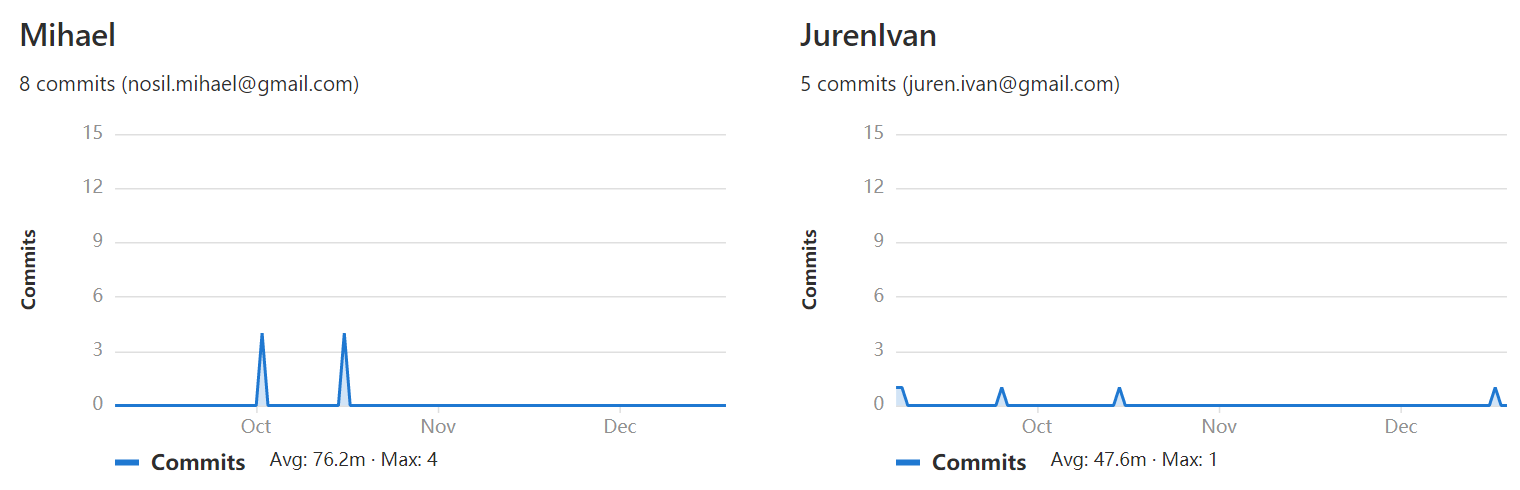
\includegraphics[width=15cm]{slike/dijagrampregledapromjena5.PNG}
			\end{center}
			\caption{Dijagram pregleda promjena po članovima tima}
			\label{fig:dijapre}
		\end{figure}
